\documentclass{article}
\usepackage{float}
\usepackage{graphicx}

\usepackage{project_440_550}
\usepackage{amsmath}
\usepackage{enumitem}
% Please submit it as is here, with line numbers.
% If you'd like a "less draft"-looking version for your website or something after:
%     \usepackage[final]{project_440_550}   % keeps the footer but kills line numbers,
%     \usepackage[preprint]{project_440_550}   % removes both


\usepackage[utf8]{inputenc} % allow utf-8 input
\usepackage[T1]{fontenc}    % use 8-bit T1 fonts

\usepackage[USenglish]{babel}  % there's a "canadian" option, but it's an alias for USenglish,
                               % and for some reason it makes csqoutes behave differently...
\usepackage{csquotes}       % smarter handling of quotes (used by biblatex)

\usepackage{booktabs}       % professional-quality tables
\usepackage{amsfonts}       % blackboard math symbols
\usepackage{nicefrac}       % compact symbols for 1/2, etc.
\usepackage{microtype}      % microtypography
\usepackage{xcolor}         % colors
\usepackage{hyperref}       % hyperlinks
\usepackage{url}            % simple URL typesetting

% I recommend the biblatex package.
% If you hate it for some reason, though, you can use natbib instead:
% comment out this block and uncomment the next one.

\usepackage[style=authoryear,maxbibnames=30,natbib]{biblatex}
\addbibresource{refs.bib}
\renewbibmacro{in:}{}  % drops a silly "In:" from biblatex format
\DeclareDelimFormat{nameyeardelim}{\addspace} % remove a comma i dislike, doesn't matter
\DeclareNameAlias{sortname}{given-family}  % avoid kinda-weird bib printing order

%\usepackage[round]{natbib}
%\newcommand{\printbibliography}{\bibliographystyle{plainnat}\bibliography{refs}}


\usepackage[capitalize,noabbrev]{cleveref}

% Inline-code macro used in tables/captions for filenames and code identifiers.
\newcommand{\code}[1]{\texttt{\small #1}}


\title{HMM-LSTM Regime Switching Model for Realized Market Volatility Prediction}


% The \author macro works with any number of authors. There are two commands
% used to separate the names and addresses of multiple authors: \And and \AND.
%
% Using \And between authors leaves it to LaTeX to determine where to break the
% lines. Using \AND forces a line break at that point. So, if LaTeX puts 3 of 4
% authors names on the first line, and the last on the second line, try using
% \AND instead of \And before the third author name.

\author{%
  Maharaj Haider\\
  \And
  West Liu\\
  \And
  Muhammad Tahir\\
  \And
    \texttt{\{mhaider0, west2020, mtahir03\}@students.cs.ubc.ca}\\
}

\begin{document}
\maketitle


\begin{abstract}
Volatility is a key driver of asset pricing and risk management, and its temporal clustering offers an opportunity for predictive models to exploit the      
  underlying structure. We test whether HMM-based regime conditioning improves over single-LSTM forecasts of 21-day-forward realized volatility on SPY, by routing predictions through      
  separate calm- and volatile-regime models. A variant-symmetric pipeline is run on sentiment inclusive and non-inclusive feature sets. For each variant, a BIC-selected       
  Gaussian-mixture HMM partitions the timeline into calm and volatile regimes; we train two regime-specific LSTMs and compare their posterior-weighted        
  ensemble against a single-LSTM baseline trained on the same features. Regime-splitting significantly beats its baseline only for the variant with sentiment and VIX-family
  inputs; on stationary or sentiment-alone-augmented features, the ensemble does not show significant differences to baseline. Decomposing within-variant gain by the HMM
  posterior state shows a calm-LSTM driven effect by specializing on calm-regime training data, and little impact from the volatile-LSTM which has collapsed to near-constant output. Regime-conditioning therefore acts as a data- and model-dependent choice, paying off only when the feature set is rich enough for the regime-specialized LSTMs to extract a meaningful per-regime edge.
\end{abstract}
\section{Introduction}

Financial market volatility measures asset price fluctuation, and is the driving factor of derivative pricing and asset risk analysis (Wang et al., 2015; Zhu \& Ling, 2015). Naturally, accurate volatility predictions help investors optimize asset allocation in attempts to derive profit. Volatility clustering, characterized by strong temporal autocorrelation in volatility, is a well-documented feature of financial markets. Early empirical evidence documents heavy-tailed return distributions and unstable variance, indicative of time-varying volatility (Mandelbrot, 1963). Econometric models such as generalized autoregressive conditional heteroskedasticity (GARCH) explicitly capture this dependence through past shocks and variance (Bollerslev, 1986). Agent-based financial market models also independently reproduce this phenomenon (Schmitt \& Westerhoff, 2016). In contrast, asset returns exhibit negligible serial correlation (Cont, 2001). This enables effective modeling of future volatility with lower frequency data (Andersen et al., 2003). 

Volatility is typically treated as a latent variable and must therefore be inferred from observed return data. In contrast, realized volatility (RV) provides a directly computable proxy by aggregating squared returns over a fixed horizon. A standard benchmark for forecasting RV is the heterogeneous autoregressive realized volatility (HAR-RV) model, a linear regression framework that predicts future volatility using lagged daily, weekly, and monthly RV components (Corsi, 2009).   Concretely, HAR-RV is the linear regression $\widehat{\sigma}_{t+h} = \beta_0 + \beta_d\,\sigma_t^{(d)} + \beta_w\,\sigma_t^{(w)} + \beta_m\,\sigma_t^{(m)}$, where $\sigma_t^{(x)}$ is the $x$-period average RV.  By explicitly incorporating these multiple time scales, HAR-RV captures the persistent, long-memory structure of volatility and is used in empirical forecasting, as a preferred reduced-form specification due to its simplicity and strong performance (Bollerslev et al., 2016).

Although HAR-RV captures persistence through lagged RV, its linear structure may limit its ability to model nonlinear relationships involving financial volatility. Evidence suggests that volatility can exhibit nonlinear interactions with other market variables, driven by factors such as heterogeneous investor behavior, transaction costs, and information frictions (Choudhry et al., 2016). Long short-term memory (LSTM) models provide a flexible alternative capable of modeling nonlinear temporal dependencies in financial time series (Pan et al., 2023). Empirical studies show that LSTM-based approaches can outperform HAR-RV in certain settings, such as agricultural stock markets (Li et al., 2025). However, these improvements are not universal, as LSTM performance depends heavily on model specification and preprocessing choices, including hyperparameter selection and input window design (He, 2026; Rodikov \& Antulov-Fantulin, 2022).

Financial markets exhibit regime-dependent behavior, with periods of low and high volatility characterized by distinct statistical properties and distributions (Cont, 2007; Guo \& Wohar, 2006). These differences motivate regime switching models, which can independently model unique heteroskedasticity, skewness, time-varying correlations, and subtle properties found in each regime (Ang \& Timmermann, 2012). Traditional models such as GARCH heavily benefit from regime-switching (Marcucci, 2005). Thus, we propose a regime-aware framework in which separate LSTM models are independently trained for each inferred market state, allowing each model to specialize its own distinct volatility learning. Our goal is to determine if regime-aware models outperform existing simple LSTM models in predicting 21-day-forward out-of-sample RV. The 21-day window is chosen to exploit the temporal clustering of volatility to obtain market leverage beyond the scope of current similar models. Regimes are inferred through Hidden Markov models (HMM) to separate markets into either high or low volatility periods (Yuan \& Mitra, 2019).
\section{Related Work}
      Regime switching has precedent and effectiveness in volatility forecasting. Marcucci (2005) establishes substantial out-of-sample gains from augmenting GARCH with Markov-chain regime-switching on US equity index returns. The model's main limitation is its rigid functional form $\sigma_t^2 = \omega + \alpha\,\varepsilon_{t-1}^2 + \beta\,\sigma_{t-1}^2$, whether regime-conditioning continues to help predict volatility when paired with a more flexible nonlinear forecaster such as an LSTM remains untested.
  
Rodikov and Antulov-Fantulin (2022) show that a tuned LSTM, trained on autoregressive sequences of lagged RV ($\mathrm{RV}_{t-n}, \dots, \mathrm{RV}_{t-1}
  \to \mathrm{RV}_t$), can outperform HAR-RV and the GARCH family on out-of-sample one-step-ahead RV forecasts across equities. Their setting differs from ours in two ways: the forecast horizon is one step ahead rather than 21 days ahead, and the LSTM
   input is restricted to lagged RV, with no price, volume, sentiment, implied-volatility, or regime-conditioning signals. Whether the single-LSTM
   continues to dominate once those are added is unknown.

Jiang et al.\ (2023) jointly train an HMM with an attention-based LSTM encoder--decoder and show that removing the HMM component degrades directional
  stock-movement forecasts. Their setting differs from ours in three ways. Firstly, the target is directional movement rather than multi-day-ahead RV. Secondly, the             
  joint-training scheme entangles the HMM regime with the LSTM's learned representations, so the reported HMM contribution may reflect interaction effects with the
  encoder--decoder rather than the regime layer alone. Finally, the input feature space is limited to OHLC prices and technical indicators, with no sentiment or VIX-family signals 
  despite evidence that such inputs carry independent predictive information for RV (Gupta et al., 2023).

Our work sits at the intersection of these three papers. We adopt the RV target of Rodikov and Antulov-Fantulin, the regime-switching motivation of        
  Marcucci, and the HMM-conditioned hybrid structure of Jiang et al., but separate the HMM and LSTM into a sequential pipeline so the regime is independently inspectable. Additionally 
  we run the regime-versus-baseline ablation across three feature-richness levels (price/volume only, with sentiment, with VIX-family inputs). This design lets us identify    
  when regime conditioning contributes and when it is absorbed by richer features.


\section{Methodology}

Our pipeline proceeds in four stages to target 21-day-ahead RV. First, we engineer a set of stationary features from raw Open-High-Low-Close-Volume (OHLCV) prices, AAII
  investor-sentiment readings, and VIX-family series. Second, an HMM is fit on these features to infer a discrete calm/volatile regime and per-day posterior
  probabilities $p_{\mathrm{calm}}$, $p_{\mathrm{vol}}$. Third, we train two regime-specialized LSTMs, one on calm-day windows, one on volatile-day windows, alongside a
  single-LSTM baseline trained on the full dataset for comparison. Fourth, at inference time the regime-LSTM forecasts are blended into an ensemble using the HMM posteriors as
   weights.

\subsection{Data}
Our forecast target is the demeaned 21-day forward RV $\sigma_t = \sqrt{(1/m)\sum_{j=1}^{m} (r_{t+j} - \bar r)^2}$ with $m=21$ (Andersen and Bollerslev, 1998), where $r_{t+j}$ are log returns and $\bar r$ is their mean over the 21-day forward window. The same target is used across all predictors, including the HAR-RV benchmark. We target SPY (SPDR S\&P~500 ETF) RV from daily OHLCV over 2001-04-01 to 2026-03-24, joined with weekly AAII sentiment (forward-filled to daily) and VIX/VIX3M closing levels. VIX-family features are included motivated by Li, Liang and Ma (2022). Asset choice rationale, feature definitions, and the chronological train/validation/test split are detailed in \cref{app:methodology-details}.

  Raw returns and volume are log-transformed to stabilize variance and produce approximately stationary inputs. We engineer multi-period rolling windows of mean and standard deviation of log returns for HMM temporal-context.
  Exploratory analysis informs correlation-pruning at a Pearson threshold of $0.95$ to keep HMM full-covariance Gaussian emissions well-conditioned (\cref{app:methodology-details}).

  The training sample size differs by variant due to data availability of VIX3M; variants O and A use $n{=}3{,}710$ training observations
  while variant B uses $n{=}2{,}034$ (2007-12 onward). Validation and test windows are identical across all variants.

  \begin{table}[H]
\centering
\caption{Variant feature sets. Variant H shares variant A's HMM; only its LSTM input is augmented. Each regime-split ensemble trains a baseline single-LSTM on the same feature set for comparison.}
\label{tab:variants}
\small
\begin{tabular}{@{}lp{4.6cm}p{4.6cm}r@{}}
\toprule
Variant & HMM input ($n_{\text{feat}}$) & LSTM input ($n_{\text{feat}}$) & Architecture \\
\midrule
\textbf{O} & price/vol $+$ rolling stats (11) & stationary returns/vol (5)              & regime-split ensemble \\
\textbf{A} & O $+$ AAII sentiment (13)         & O $+$ AAII sentiment (7)                  & regime-split ensemble \\
\textbf{H} & shares A's HMM                    & A $+$ HMM posterior $p_{\text{vol}}$ (8)  & single LSTM \\
\textbf{B} & A $+$ VIX family (16)             & A $+$ VIX family (10)                     & regime-split ensemble \\
\bottomrule
\end{tabular}
\end{table}

\subsection{HMM regime detection}

  For each HMM variant we fit Gaussian and Gaussian-mixture HMM (GMMHMM) emissions with 2 hidden states and full covariance, sweeping $n_{\text{mix}} \in \{1, 2, 3\}$, and select the winner by
  validation BIC. Mixture emissions are preferred to single-Gaussian on both validation BIC and data-distribution grounds (Zhang et al., 2019; \cref{app:hmm-checks}, \cref{app:gmmhmm-rationale}). Training uses 50 random restarts with a penalized-likelihood criterion (Nystrup et al., 2017) to suppress degenerate rapid-switching solutions (\cref{app:methodology-details}). The post-hoc volatile state is identified by which state has the larger
  absolute log mean return $|r_t|$ on the training set. Inference uses Viterbi for hard labels and the forward--backward algorithm for soft probabilities. As robustness checks we additionally tested a second-order Markov approximation (state- and feature-space augmentation; Lee, 2017) and a 3-state extension; neither beat the first-order 2-state winner by the BIC margin we set to justify the added complexity (\cref{app:hmm-checks}).

  \subsection{LSTM training}
Each LSTM is a multi-layer LSTM with a single linear output head, trained to predict the log-transformed forecast target with predictions exponentiated back to the original
  scale for evaluation. Inputs are standardized with a StandardScaler fit on training data only to prevent leakage. Optimization uses Adam with an MSE loss and
  validation-MSE-based early stopping. Hyperparameters (hidden size, number of layers, dropout, learning rate, batch size, sequence length) are selected per variant by Optuna's tree-structured Parzen estimator (Akiba et al., 2019) over a 20-trial budget on the validation split. To absorb single-seed run-to-run variance we train each LSTM with $k=3$ random seeds (42, 43, 44) and report the cross-seed mean prediction (\cref{app:methodology-details}).

    \subsection{Regime-conditioned ensemble}
    \label{sec:methodology-ensemble}

  Variants O, A, and B each train two additional regime-specific LSTMs, one for each of the calm and volatile states inferred by the variant's HMM. Regime-specific training uses windows whose dominant Viterbi label matches the target regime. At inference, the calm- and volatile-LSTM forecasts are combined by the HMM's forward--backward soft probabilities at time $t$ as $\hat\sigma_t = P(\text{calm} \mid O_{1:T})_t \cdot \hat\sigma^{\,\text{calm}}_t + P(\text{volatile} \mid O_{1:T})_t \cdot \hat\sigma^{\,\text{vol}}_t$. Variant H is the exception: it consumes the HMM posterior $p_{\text{volatile}}$ as an additional input feature to a single LSTM, testing whether the regime signal can be exploited through feature augmentation rather than ensemble specialization.


  \subsection{Comparison protocol}

We compare each variant's regime-split ensemble against its baseline LSTM via the Diebold--Mariano test (DM) (Rodikov \& Antulov-Fantulin, 2022), two-sided on both squared (MSE) and absolute (MAE) error loss series. Cross-variant comparisons across the six predictors (four ensembles, persistence (\code{rolling\_std\_21}), and HAR-RV) give 30 DM tests; false positives are controlled by Benjamini--Hochberg FDR (Benjamini \& Hochberg, 1995). HAR-RV (Corsi, 2009) is fit on the training split. Small-sample correction, HAC bandwidth, and HAR-RV target-formula adaptation are detailed in \cref{app:methodology-details} and \cref{app:harrv}.

\section{Analysis}
\label{sec:analysis}

We evaluate all six predictors (4 variant LSTMs, naive, and HAR-RV benchmark) on a row-aligned common test index of $n = 1{,}440$ trading days (2020-06-30 to 2026-03-24) where all predictors produce a valid forecast (after the longest 42-day LSTM warmup).

\subsection{Raw and within-variant performance}

Three tiers of MAPE separate cleanly across the predictors (\cref{tab:headline}, \cref{app:headline}): the richer-feature variants A and B (with sentiment inputs) and H (with regime-probability input) cluster at $24$--$26\%$, variant O and HAR-RV sit at $30$--$31\%$, and the naive persistence baseline at $34.6\%$. The largest single-feature contribution is sentiment: the O to A transition reduces MAPE by $5.9$ pp. At the cross-variant level, BH-FDR-corrected DM tests confirm that A, B, and H each significantly beat both naive and HAR-RV on MAE (raw $p \le 0.001$; \cref{tab:cross-dm}, \cref{app:cross-dm}), while pairwise differences within the top tier (A vs B, A vs H, B vs H) do not reject.

The core question of our research focuses on whether \emph{regime-splitting} adds value over a single-LSTM baseline trained on the same features. We perform within-variant DM tests for each of the three regime-split variants (\cref{tab:within}, \cref{app:within}). The regime-splitting hypothesis is supported only for variant B, the model trained on stationary features, sentiment, and VIX-family inputs. The ensemble significantly outperforms its baseline on both losses. The hypothesis is therefore more accurately stated as a feature-interaction idea: the value of regime-conditioning depends on the extent to which the LSTMs have features whose distribution differs across regimes. Variant B is trained on a richer feature set (sentiment plus VIX-family inputs) that variants O and A lack; \cref{sec:vol-lstm-degen} examines the underlying mechanism. That said, the $p_{\mathrm{MAE}}$ values for variants O and A ($0.07$ and $0.06$) are borderline, so a marginal benefit cannot be ruled out.

\subsection{The persistence-shift floor}
\label{sec:persistence-shift}

Variants O, A, H, and B all improve over the naive persistence baseline on point-error metrics, but none of them eliminates a structural lag in the cross-correlation between predictions and target. We define the \emph{persistence-shift floor} operationally: let $\ell^\star_p$ be the lag at which a predictor $p$'s test-window cross-correlation $\mathrm{corr}(p_t, y_{t+\ell})$ peaks. The naive baseline $p_t = \sigma_{t-21:t}$ has $\ell^\star = -21$ by construction; a perfect contemporaneous predictor would have $\ell^\star = 0$. The persistence-shift floor is the smallest $|\ell^\star|$ achieved by any model in our search space: the number of days of trailing return data the best learned model is still effectively replaying.

Empirically, the floor sits at $|\ell^\star| = 16\text{--}17$ for every learned variant, four to five days closer to zero than naive but never reaching it (\cref{fig:f0}, \cref{fig:f1}, \cref{app:f1}). HAR-RV inherits the naive peak at $\ell^\star = -21$ through its dominant 21-day backward component. Lag-zero correlation improves with richer features ($0.46$ naive $\to 0.60$ variant A), but the dominant signal remains the trailing $16$--$17$ days of data. Improvement would require either higher-frequency inputs or a shorter forecast horizon.

\begin{figure}[!t]
\centering
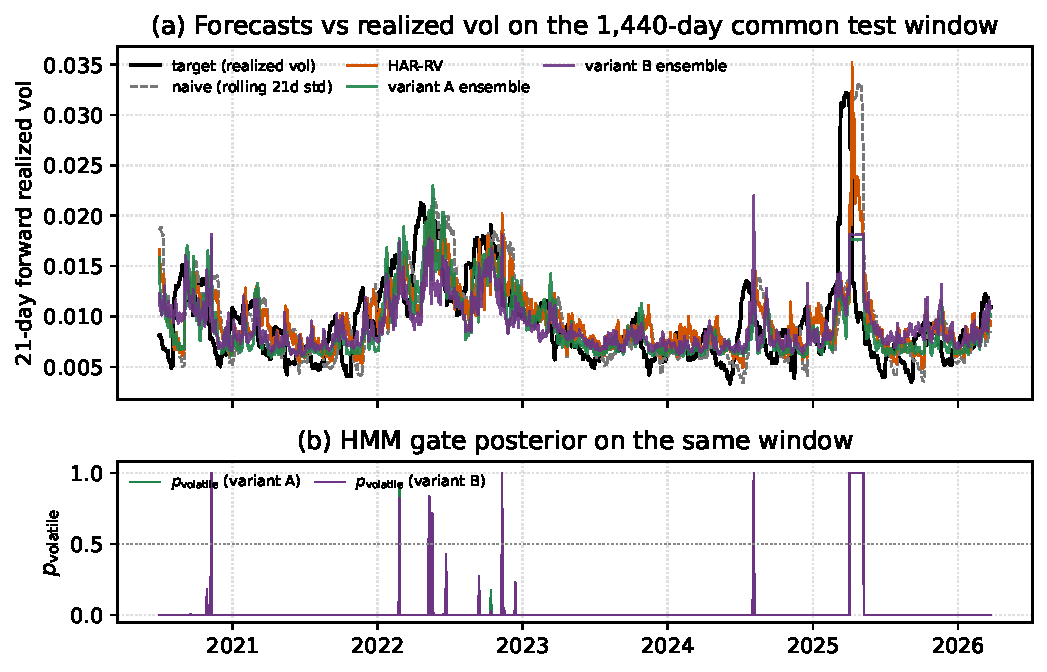
\includegraphics[width=\linewidth]{figures/F0_main_panel.pdf}
\caption{Forecast trajectories and HMM posterior on the 1{,}440-day common test window. \textbf{(a)} RV target (black) against naive, HAR-RV, and variant A and B regime-split ensembles (3-seed means); the visible right-shift of every learned curve is the persistence-shift lag of \cref{sec:persistence-shift}. \textbf{(b)} $p_{\mathrm{volatile}}$ for variants A and B; both spend the bulk of the window near zero and concentrate volatile mass on the March--April 2025 spike.}
\label{fig:f0}
\end{figure}

\subsection{Volatile-LSTM degeneracy is masked by the posterior weighting}
\label{sec:vol-lstm-degen}

The per-seed volatile-LSTM outputs look pathological in two of three variants (\cref{tab:f2}, \cref{app:f2}). Variant A explodes with prediction standard deviations  up to 195 times larger than the target standard deviation ($\sigma_{\mathrm{tgt}} = 0.0044$). Conversely, variant B collapses to a near-constant at worst $4.2 \times 10^{-4}$ smaller than the target. Variant O is well-behaved (std $0.0031$--$0.0038$), which is reasonable given its much larger volatile training bucket of $n_{\mathrm{vol}} = 2{,}495$ days against ${\sim}\,200$ for A and B (\cref{tab:regime-dist}).

These behaviors are largely absorbed by the posterior-weighted blend $\hat\sigma_t = p_{\mathrm{calm}}(t) \cdot \hat\sigma^{\mathrm{calm}}_t + p_{\mathrm{volatile}}(t) \cdot \hat\sigma^{\mathrm{vol}}_t$. The variant-A explosions occur only on calm days, where $p_{\mathrm{volatile}}$ has mean $0.0002$, median $0$, and 95th percentile $0$, so the volatile-LSTM contribution to the ensemble has mean ${\approx}\,0$ and maximum $0.003$, below $\sigma_{\mathrm{tgt}}$ even at its worst. On the rare crisis days where $p_{\mathrm{volatile}}$ rises (28 days for A, 34 for B with $p_{\mathrm{volatile}} \geq 0.5$), both variants' volatile LSTMs have collapsed to a near-constant ${\sim}\,0.018$, which sits closer to typical crisis-day targets (mean $0.014$) than the baseline LSTM's calm-biased prediction. The variant-B within-variant DM rejection in \cref{tab:within} therefore comes mostly from the calm LSTM out-predicting the baseline on calm days, with a smaller crisis-day contribution from the constant-${\sim}\,0.018$ fallback. The regime-split architecture works less because the volatile LSTM is a competent crisis forecaster and more because the small $p_{\mathrm{volatile}}$ on most days hides its degeneracy from the ensemble. This volatile-LSTM mode-flip is also the largest single driver of cross-seed variance: variant B has a $13.5\%$ MSE coefficient of variation against $3$--$7\%$ for O/A/H (\cref{tab:cv}, \cref{app:cv}), so the variant-B rejection could plausibly invert under different seed selection.

\subsection{Accessory probe: GaussianHMM emission on variants O, A, B (variants Os, As, Bs)}
\label{sec:os-discovery}

Variant O's BIC-optimal GMMHMM ($n_{\mathrm{mix}}=3$) failed to find a persistent regime basin: $p_{\mathrm{volatile}}$ flips between $0$ and $1$ on a near-daily basis (\cref{fig:variant-O-diag}, \cref{fig:pvol}), inconsistent with the regime-persistent structure of volatility clustering. A duration-penalty sweep on the transition matrix did not recover persistence at any tested value. Refitting the same 11 features with a plain GaussianHMM emission, which we call variant \emph{Os} (``O simple''), yields a regime-persistent partition (autocorrelation $0.97$) and drops ensemble MAPE from $30.14\%$ to $23.48\%$, the lowest of all seven predictors and competitive with variant A (\cref{tab:os-probe}, \cref{app:os-probe}).

We did not find a comparable advantage when applying the same emission swap to variants A and B (variants \emph{As} and \emph{Bs}; \cref{fig:f5}, \cref{app:emission-comp}). A's and B's HMM feature sets contain inputs that are themselves regime-discriminating (sentiment in A, VIX-family in B), which anchor the BIC-optimal partition along the regime axis even under mixture emissions. Variant O's feature set lacks any such anchor, so the additional within-state mixture capacity is instead spent fitting non-regime distributional structure (heavy tails, fine-grained density shape) at the cost of regime persistence; restricting variant O to a single-Gaussian emission removes that misallocated capacity and forces the partition onto the coarsest available axis of separation, which empirically aligns with the regime structure. The rescue is therefore specific to variant O's broken fit.

\section{Discussion and Future Work}
\label{sec:discussion}

The regime-switching ensemble outperforms its single-LSTM baseline only for variant B, the variant with the richest forward-looking inputs (VIX-family). The selectivity of this result reframes the regime-switching hypothesis as a feature-interaction claim: regime-conditioning shows promise but is heavily input- and model-dependent. Both the model inputs and the choice of HMM emission class shape the regime assignment: variant O's original GMMHMM failed to find a persistent regime basin and produced a near-daily flip-flop in $p_{\mathrm{volatile}}$ until the emission was simplified to a plain Gaussian. The volatile LSTM, in turn, collapsed to a near-constant under the small ${\sim}200$-day volatile training bucket common to variants A and B, so the variant-B improvement is carried mostly by the calm LSTM specializing on the calm-regime input distribution and out-predicting the all-data baseline, not by the volatile LSTM itself.

On the feature side, sentiment substantially improves absolute prediction quality across all variants but does not flip any within-variant DM verdict. The persistence-shift floor at $\sim 17$ days is the more concerning structural finding: every learned predictor effectively replays trailing return data from $16$--$17$ days ago, four to five days closer to the present than the naive baseline but never reaching it. This reflects the limits of daily-frequency inputs against a 21-day-forward target. Higher-frequency data would directly probe whether the floor scales with the input-to-horizon ratio, and would also enlarge the effective volatile-state training bucket, thereby mitigating the data-scarcity collapse that broke the volatile LSTM in this work.

The strength of this work is the rigour and breadth of the comparison itself. The rigid variant-symmetric pipeline isolates the regime-conditioning effect from feature effects, the full chain of data-distribution diagnostics, BIC-based model selection, and per-variant Optuna hyperparameter searches removes tuning and model-class confounds, and adjusted significance tests (DM with HLN small-sample correction and Bartlett HAC, plus Benjamini--Hochberg FDR control) yield fair per-variant verdicts. The principal weakness is data availability. Daily SPY across twenty years is enough to train a 21-day-forward volatility forecaster but it does not give the volatile-regime LSTM enough crisis days to be a real predictor; the same constraint closes off adjacent problems such as stock-price prediction, whose data requirements are substantially harder to meet with our current scale of resources.

The most useful extensions are in the data. Expanding the input set in frequency, such as intraday hourly or minute-bar returns, and breadth (daily news-sentiment analysis as opposed to weekly) would directly enlarge the volatile-regime training bucket and probe whether the persistence-shift floor scales with the input-to-horizon ratio. Beyond that, running the same regime-conditioned framework across separate markets or sub-markets is worth pursuing: there is no \emph{a priori} reason that the 2008 financial-crisis volatility regime and the 2020 pandemic regime should look the same, so training and predicting on narrower, more concentrated volatility windows may extract per-regime structure that whole-history models smooth over.


\section*{References}

\small
\begin{description}[leftmargin=1.5em,labelindent=0pt,style=unboxed,itemsep=0.2em,topsep=0.2em]

\item Akiba, T., Sano, S., Yanase, T., Ohta, T., \& Koyama, M. (2019). Optuna: A next-generation hyperparameter optimization framework. In \emph{Proceedings of the 25th ACM SIGKDD International Conference on Knowledge Discovery \& Data Mining} (pp.\ 2623--2631).

\item Andersen, T.~G., \& Bollerslev, T. (1998). Answering the skeptics: Yes, standard volatility models do provide accurate forecasts. \emph{International Economic Review}, 39(4), 885--905.

\item Andersen, T.~G., Bollerslev, T., Diebold, F.~X., \& Labys, P. (2003). Modeling and forecasting realized volatility. \emph{Econometrica}, 71(2), 579--625.

\item Ang, A., \& Timmermann, A. (2012). Regime changes and financial markets. \emph{Annual Review of Financial Economics}, 4(1), 313--337.

\item Benjamini, Y., \& Hochberg, Y. (1995). Controlling the false discovery rate: A practical and powerful approach to multiple testing. \emph{Journal of the Royal Statistical Society: Series B (Methodological)}, 57(1), 289--300.

\item Bollerslev, T. (1986). Generalized autoregressive conditional heteroskedasticity. \emph{Journal of Econometrics}, 31(3), 307--327.

\item Bollerslev, T., Patton, A.~J., \& Quaedvlieg, R. (2016). Exploiting the errors: A simple approach for improved volatility forecasting. \emph{Journal of Econometrics}, 192(1), 1--18.

\item Choudhry, T., Papadimitriou, F.~I., \& Shabi, S. (2016). Stock market volatility and business cycle: Evidence from linear and nonlinear causality tests. \emph{Journal of Banking \& Finance}, 66, 89--101.

\item Cont, R. (2001). Empirical properties of asset returns: Stylized facts and statistical issues. \emph{Quantitative Finance}, 1(2), 223--236.

\item Cont, R. (2007). Volatility clustering in financial markets: Empirical facts and agent-based models. In \emph{Long Memory in Economics} (pp.\ 289--309). Springer.

\item Corsi, F. (2009). A simple approximate long-memory model of realized volatility. \emph{Journal of Financial Econometrics}, 7(2), 174--196.

\item Gupta, R., Nel, J., \& Pierdzioch, C. (2023). Investor confidence and forecastability of US stock market realized volatility: Evidence from machine learning. \emph{Journal of Behavioral Finance}, 24(1), 111--122.

\item Guo, W., \& Wohar, M.~E. (2006). Identifying regime changes in market volatility. \emph{Journal of Financial Research}, 29(1), 79--93.

\item Harvey, D., Leybourne, S., \& Newbold, P. (1997). Testing the equality of prediction mean squared errors. \emph{International Journal of Forecasting}, 13(2), 281--291.

\item He, Y. (2026). Forecasting stock market volatility: A comparison of GARCH, HAR-RV, and LSTM models. Working paper, March 9, 2026.

\item Jiang, J., Wu, L., Zhao, H., Zhu, H., \& Zhang, W. (2023). Forecasting movements of stock time series based on hidden state guided deep learning approach. \emph{Information Processing \& Management}, 60(3), 103328.

\item Lee, J. (2017). \emph{Multi-level hidden Markov model and ULSTM network} (PhD thesis). Seoul National University.

\item Li, H., Huang, X., Luo, F., Zhou, D., Cao, A., \& Guo, L. (2025). Revolutionizing agricultural stock volatility forecasting: A comparative study of machine learning and HAR-RV models. \emph{Journal of Applied Economics}, 28(1), 2454081.

\item Li, X., Liang, C., \& Ma, F. (2022). Forecasting stock market volatility with a large number of predictors: New evidence from the MS-MIDAS-LASSO model. \emph{Annals of Operations Research}, 352(3), 613--652. \url{https://doi.org/10.1007/s10479-022-04716-1}

\item Mandelbrot, B. (1963). The variation of certain speculative prices. \emph{Journal of Business}, 36(4), 394--419.

\item Marcucci, J. (2005). Forecasting stock market volatility with regime-switching GARCH models. \emph{Studies in Nonlinear Dynamics \& Econometrics}, 9(4), 1--53.

\item Nystrup, P., Madsen, H., \& Lindstr\"om, E. (2017). Long memory of financial time series and hidden Markov models with time-varying parameters. \emph{Journal of Forecasting}, 36(8), 989--1002.

\item Pan, S., Long, S.~C., Wang, Y., \& Xie, Y. (2023). Nonlinear asset pricing in Chinese stock market: A deep learning approach. \emph{International Review of Financial Analysis}, 87, 102627.

\item Rodikov, G., \& Antulov-Fantulin, N. (2022). Can LSTM outperform volatility-econometric models? arXiv preprint arXiv:2202.11581.

\item Schmitt, N., \& Westerhoff, F. (2016). Speculative behavior and the dynamics of interacting stock markets. \emph{Journal of Economic Dynamics and Control}, 45, 262--288.

\item Wang, X., Wu, C., \& Xu, W. (2015). Volatility forecasting: The role of lunch-break returns, overnight returns, trading volume and leverage effects. \emph{International Journal of Forecasting}, 31(3), 609--619. \url{https://doi.org/10.1016/j.ijforecast.2014.10.007}

\item Yuan, Y., \& Mitra, G. (2019). Market regime identification using hidden Markov models (SSRN Working Paper No.\ 3406068). \url{https://doi.org/10.2139/ssrn.3406068}

\item Zhang, M., Jiang, X., Fang, Z., Zeng, Y., \& Xu, K. (2019). High-order hidden Markov model for trend prediction in financial time series. \emph{Physica A: Statistical Mechanics and its Applications}, 517, 1--12.

\item Zhu, K., \& Ling, S. (2015). Model-based pricing for financial derivatives. \emph{Journal of Econometrics}, 187(2), 447--457. \url{https://doi.org/10.1016/j.jeconom.2015.02.030}

\end{description}
\normalsize

%%%%%%%%%%%%%%%%%%%%%%%%%%%%%%%%%%%%%%%%%%%%%%%%%%%%%%%%%%%%

\appendix
\raggedbottom

\section{Supplementary Material}
\label{app:info}

\subsection{Methodology details}
\label{app:methodology-details}

\paragraph{Asset, supplementary features, and chronological split (\S 3.1).} SPY (SPDR S\&P~500 ETF) is chosen as a broad-market proxy: it tracks the S\&P 500 index and so its realized volatility reflects aggregate US equity-market volatility. The supplementary inputs are AAII weekly investor-sentiment readings (a non-price sentiment signal that is independent of price-action features) and the CBOE VIX and VIX3M closing levels, which are the 30-day and 3-month implied-volatility indices priced from S\&P 500 options and act as forward-looking volatility expectations from the options market. The chronological split is fixed across all variants: training spans 2001-04-01 to 2015-12-31 ($n_{\text{train}} = 3{,}710$ trading days, or $n = 2{,}034$ for variant B due to VIX3M's later 2007-12-04 inception), validation spans 2016-01-01 to 2019-12-31, and test spans 2020-01-01 to 2026-03-24 (with the first ${\sim}42$ test days dropped to the LSTM warmup, leaving the 1{,}440-day common test index used throughout the paper).

\paragraph{Feature engineering: collinearity threshold (\S 3.1).} The 0.95 Pearson threshold is a pragmatic heuristic that removes near-redundant inputs which would produce ill-conditioned or singular sample covariance matrices in the HMM's full-covariance Gaussian emissions; weaker collinearity that survives the prune is not eliminated, but is partially absorbed by hmmlearn's default Bayesian regularization of the EM covariance update and a hard floor on diagonal entries, which together keep training numerically stable in practice.

\paragraph{HMM regularization: penalized likelihood (\S 3.2).} We use 50 random restarts with the Nystrup et al.\ (2017) penalized-likelihood criterion
\[
\mathcal L_{\text{pen}} \;=\; \log P(O \mid \theta) \;-\; \lambda \sum_{s} \bigl(1 - p_{ss}\bigr),
\]
with $\lambda = 3{,}000 \approx n_{\text{train}}$, to suppress degenerate rapid-switching solutions.

\paragraph{LSTM seed strategy and Optuna reuse (\S 3.3).} Following our preliminary analysis showing single-seed LSTM metrics swing by $>50\%$ across reruns with identical configuration, we train each LSTM with $k=3$ random seeds (42, 43, 44). Seed 42 runs the full Optuna search and persists the resulting hyperparameters; seeds 43 and 44 reuse those hyperparameters and only retrain, saving compute without biasing the cross-seed variance estimate, since the dominant noise source is weight initialization and CPU floating-point non-determinism rather than Optuna trial order.

\paragraph{DM protocol details (\S 3.5).} The DM test uses the Harvey--Leybourne--Newbold small-sample correction and a Bartlett HAC variance estimator at lag $h{-}1 = 20$ (Harvey, Leybourne, \& Newbold, 1997). The 15 cross-variant pairs among the six predictors give 30 tests when run on both MSE and MAE loss series. The 1{,}440-day common test index is the intersection of dates on which every predictor has a valid forecast (i.e.\ after the longest 21- or 42-day LSTM warmup).

\subsection{HMM model selection and topology robustness checks}
\label{app:hmm-checks}

Each HMM variant was selected from the candidate set $\{$GaussianHMM, GMMHMM$(n_{\text{mix}}=2)$, GMMHMM$(n_{\text{mix}}=3)\}$ at fixed $n_{\text{states}}=2$ and full covariance, using validation BIC (lower is better). On variant A's feature set, GMMHMM$(n_{\text{mix}}=2)$ won by $\sim 14$k BIC over GMMHMM$(n_{\text{mix}}=3)$ and by $>34$k over single-Gaussian. Under their own feature sets, variants A and B selected GMMHMM$(\text{states}=2, \text{mix}=2)$, while variant O selected GMMHMM$(\text{states}=2, \text{mix}=3)$. This fits the misallocated-mixture-capacity mechanism in \cref{sec:os-discovery}: variant O's feature set has no regime-discriminating anchor, so the EM optimizer makes use of the additional within-state mixture flexibility. We additionally tested second-order Markov dependence above the BIC-selected first-order winner, via both state-space augmentation ($S^2 = 4$ composite states) and feature-space augmentation (lagged observations appended); neither beat the first-order winner by the 10-nat BIC margin we set to justify the added complexity. As a robustness check on the choice of $n_{\text{states}} = 2$ we re-ran the full sweep at $n_{\text{states}} = 3$ on variant O's 11-feature input; the three-state $\mathrm{GMMHMM}(n_{\text{states}}=3, n_{\text{mix}}=2)$ was BIC-inferior to the two-state winner by $\sim 3{,}600$ nats, and its Viterbi assignment further showed that the ``calm'' state contained only $1$ training observation out of $3{,}690$, effectively collapsing to a two-state partition with one redundant state.

\subsection{GMMHMM rationale: feature non-normality and collinearity}
\label{app:gmmhmm-rationale}

The BIC sweep in \cref{app:hmm-checks} prefers the mixture-emission HMM by a wide margin ($\mathrm{GMMHMM}(n_{\mathrm{mix}}=2)$ wins by ${>}34$k nats over single-Gaussian under variant A's feature set). \cref{fig:gmmhmm-rationale} shows the data-side evidence supporting that same conclusion.

Panel (a) is the Q-Q plot of training-window SPY log returns against the standard normal. The empirical quantiles peel away from the dashed reference line in both tails, with skew $-0.05$, excess kurtosis $+11.3$, and Jarque--Bera $p = 0$ to floating-point precision. A single-Gaussian state distribution would assign exponentially-vanishing density to the tails the data routinely visit, so the volatile state would underfit precisely the crisis days the HMM is meant to flag. A mixture of $n_{\mathrm{mix}} = 2$ Gaussians per state has the flexibility to absorb the leptokurtic tail mass while keeping the bulk near the modal Gaussian, which is the analytic justification behind the BIC verdict.

Panel (b) is the Pearson correlation matrix of variant B's 16 HMM input features on the training window. Two structural blocks dominate: the rolling-volatility cluster (\code{rolling\_std\_5/10/21}, $\rho$ up to $0.94$) and the VIX/rolling-vol block ($\rho$ up to $0.91$). All pairwise $|\rho|$ sit under the $0.95$ pruning threshold (\cref{app:methodology-details}) so no features are dropped, but enough collinearity survives that a single-Gaussian state with full $16{\times}16$ covariance would inherit a near rank-deficient EM update. The mixture decomposition splits each state's mass across two Gaussians whose component covariances need only model the within-component spread, which empirically gives more stable EM convergence on the same feature set.

\begin{figure}[H]
\centering
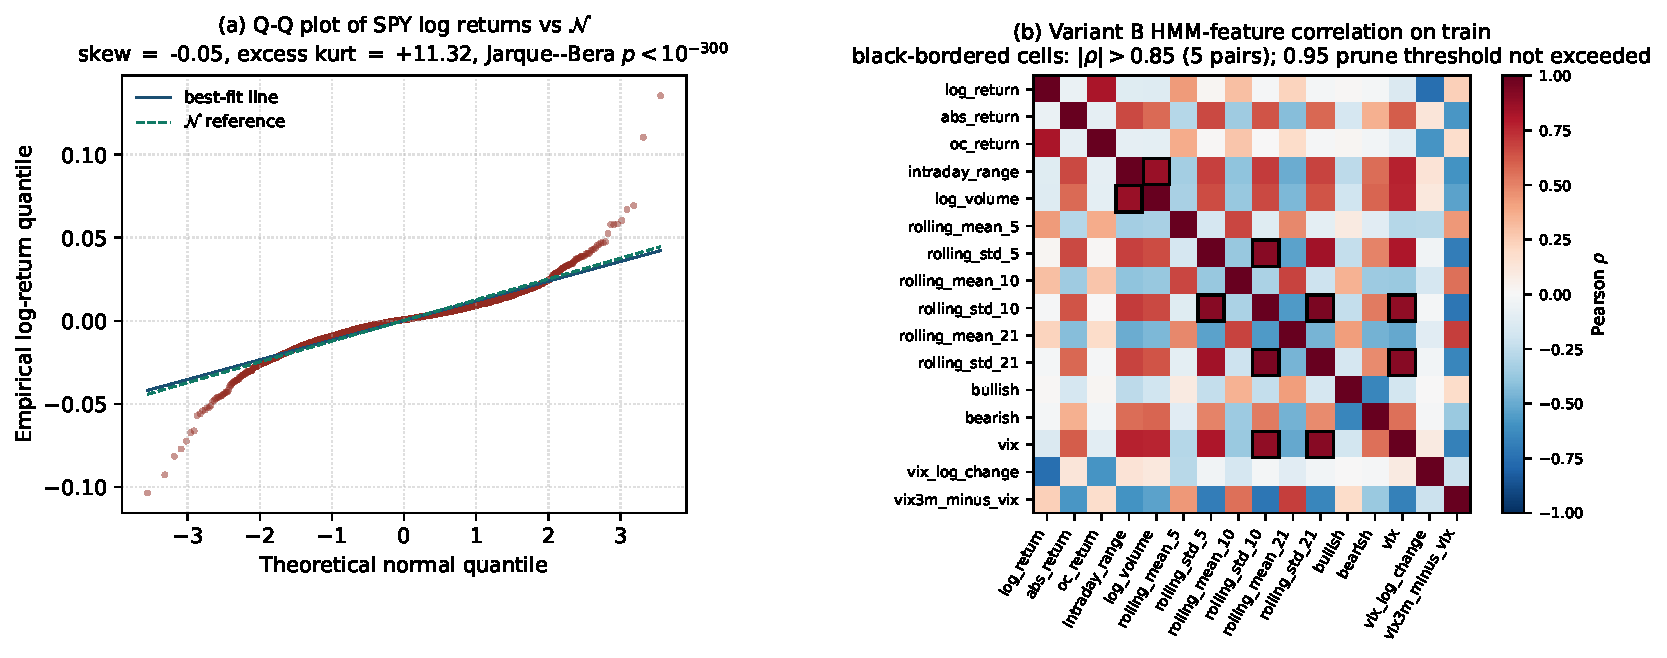
\includegraphics[width=\linewidth]{figures/F_gmmhmm_rationale.pdf}
\caption{GMMHMM rationale on the training window. \textbf{(a)} Q-Q plot of SPY log returns against $\mathcal{N}$; tails diverge sharply from the dashed reference line, with excess kurtosis $+11.3$. \textbf{(b)} Variant B HMM-feature correlation matrix; the rolling-vol and VIX blocks reach $|\rho| \approx 0.94$, all under the $0.95$ pruning threshold but indicative of remaining structure that single-Gaussian full-covariance emissions handle poorly.}
\label{fig:gmmhmm-rationale}
\end{figure}

\subsection{HAR-RV target-formula adaptation}
\label{app:harrv}

We use HAR-RV (Corsi, 2009) adapted to our forward-21-day target. The original Corsi formulation predicts one-day-ahead realized volatility; we predict the same forward 21-day realized volatility used by the LSTMs:
\[
\sigma_{t} \;=\; c \;+\; \beta_d \cdot RV_d(t) \;+\; \beta_w \cdot RV_w(t) \;+\; \beta_m \cdot RV_m(t) \;+\; \varepsilon_t,
\]
where $\sigma_t$ is the forward-21-day realized volatility target and $RV_d, RV_w, RV_m$ are backward-looking realized-volatility components at 1-, 5-, and 21-day horizons. The 1-day component is $|r_t|$ (un-demeaned, since demeaning a single observation is degenerate, matching Corsi's convention); the 5- and 21-day components use the same demeaned formula as the target. Fitted coefficients on the train split are $(c, \beta_d, \beta_w, \beta_m) = (+0.0027, +0.046, +0.234, +0.494)$. The dominance of $\beta_m$ explains why HAR-RV peaks at the same lag $-21$ as naive in \cref{fig:f1}: HAR-RV is essentially a bias-corrected version of the persistence baseline.

\subsection{Headline metrics}
\label{app:headline}

\begin{table}[H]
\centering
\caption{Test-set metrics on the common 1{,}440-row index, mean across 3 seeds. Bolded cells are best per metric across the four main variants and two non-deep baselines.}
\label{tab:headline}
\small
\begin{tabular}{@{}lcccc@{}}
\toprule
Predictor & MSE & RMSE & MAE & MAPE \\
\midrule
naive ($\sigma_{t-21}$)                & $2.20\!\times\!10^{-5}$ & $0.00469$ & $0.00313$ & $34.59\%$ \\
HAR-RV (Corsi, 2009)                   & $1.61\!\times\!10^{-5}$ & $0.00401$ & $0.00278$ & $31.26\%$ \\
variant O (ensemble)                   & $1.43\!\times\!10^{-5}$ & $0.00378$ & $0.00264$ & $30.14\%$ \\
\textbf{variant A (ensemble)}          & $1.30\!\times\!10^{-5}$ & $0.00360$ & $\mathbf{0.00235}$ & $\mathbf{24.23\%}$ \\
variant H (baseline)                   & $1.38\!\times\!10^{-5}$ & $0.00372$ & $0.00243$ & $24.91\%$ \\
\textbf{variant B (ensemble)}          & $\mathbf{1.29\!\times\!10^{-5}}$ & $\mathbf{0.00359}$ & $0.00239$ & $25.51\%$ \\
\bottomrule
\end{tabular}
\end{table}

\subsection{Within-variant DM table}
\label{app:within}

\begin{table}[H]
\centering
\caption{Within-variant DM tests: regime-split ensemble vs single-LSTM baseline within the \emph{same} feature pipeline. Positive DM means the ensemble wins. Verdicts at $\alpha = 0.05$ on raw $p$.}
\label{tab:within}
\small
\begin{tabular}{@{}lcccccl@{}}
\toprule
Variant & DM$_{\mathrm{MSE}}$ & $p_{\mathrm{MSE}}$ & DM$_{\mathrm{MAE}}$ & $p_{\mathrm{MAE}}$ & $n$ & Verdict ($\alpha=0.05$) \\
\midrule
O          & $+0.14$           & $0.89$            & $-1.79$           & $0.07$            & 1{,}440 & no rejection \\
A          & $+1.46$           & $0.15$            & $+1.92$           & $0.06$            & 1{,}440 & no rejection \\
\textbf{B} & $\mathbf{+2.17}$  & $\mathbf{0.030}$  & $\mathbf{+2.25}$  & $\mathbf{0.025}$  & 1{,}440 & \textbf{ensemble wins} \\
\bottomrule
\end{tabular}
\end{table}

\subsection{Cross-variant DM table (BH-FDR-corrected)}
\label{app:cross-dm}

Of the 30 pairwise tests across the 6 predictors $\times$ 2 loss functions, 9 reject under BH-FDR at $\alpha = 0.05$ (\cref{tab:cross-dm}). Variants A, B, and H form a top tier (significantly beating naive and HAR-RV on MAE) and are statistically indistinguishable from each other in pairwise comparisons.

\begin{table}[H]
\centering
\caption{Cross-variant DM tests rejecting under Benjamini--Hochberg FDR ($\alpha = 0.05$). Sorted by raw $p$-value ascending. Positive DM means the second-listed predictor wins.}
\label{tab:cross-dm}
\small
\begin{tabular}{@{}llcccl@{}}
\toprule
Predictor 1 & Predictor 2 & loss & DM & raw $p$ & Verdict \\
\midrule
HAR-RV               & variant A (ens.)  & MAE & $+4.01$ & $0.0001$ & A wins \\
naive                & variant A (ens.)  & MAE & $+3.85$ & $0.0001$ & A wins \\
naive                & variant H (base.) & MAE & $+3.59$ & $0.0003$ & H wins \\
variant O (ens.)     & variant A (ens.)  & MAE & $+3.49$ & $0.0005$ & A wins \\
HAR-RV               & variant H (base.) & MAE & $+3.45$ & $0.0006$ & H wins \\
naive                & variant B (ens.)  & MAE & $+3.42$ & $0.0006$ & B wins \\
HAR-RV               & variant B (ens.)  & MAE & $+3.32$ & $0.0009$ & B wins \\
variant O (ens.)     & variant B (ens.)  & MAE & $+2.92$ & $0.0036$ & B wins \\
naive                & HAR-RV            & MAE & $+2.68$ & $0.0074$ & HAR-RV wins \\
\bottomrule
\end{tabular}
\end{table}

\subsection{Cross-correlation profile (the persistence-shift floor)}
\label{app:f1}

\begin{figure}[H]
\centering
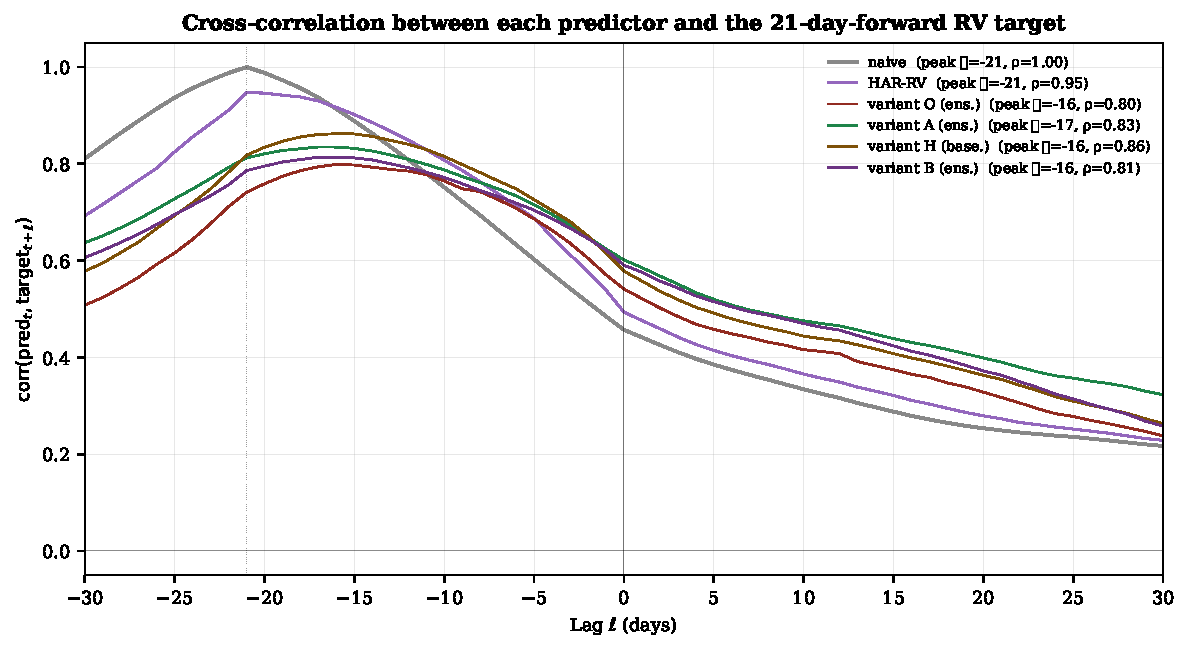
\includegraphics[width=0.78\linewidth]{figures/F1_cross_correlation_profile.pdf}
\caption{Cross-correlation profile of each predictor against the target across lags $\ell \in [-30, +30]$. A peak at $\ell = -k$ means the prediction lags the target by $k$ days; a perfect contemporaneous predictor would peak at $\ell = 0$. The naive baseline peaks at $\ell = -21$ with correlation $1.00$ (by construction); HAR-RV inherits the same peak through its dominant 21-day backward component. Each learned variant (O, A, H, B) peaks at $\ell = -16$ to $-17$, four to five days closer to zero than naive but never reaching it. We refer to this gap as the \emph{persistence-shift floor} (\cref{sec:persistence-shift}).}
\label{fig:f1}
\end{figure}

\subsection{Per-seed volatile-LSTM prediction statistics}
\label{app:f2}

\begin{table}[H]
\centering
\caption{Volatile-regime LSTM prediction statistics by variant and seed; target std on the common test index is $0.0044$. Variant A consistently explodes across seeds, variant B mostly collapses with one partial-explosion seed, and variant O is the only configuration whose volatile LSTM behaves consistently like a real predictor (the variant-dependent failure modes traced in \cref{sec:vol-lstm-degen}). The ``range'' column is $\max - \min$ (window span), not an interval.}
\label{tab:f2}
\small
\begin{tabular}{@{}lcrrrl@{}}
\toprule
Variant & Seed & pred std & range & std / target & Note \\
\midrule
A & 42 & $0.732$  & $2.72$  & $165\times$  & wildly non-stationary \\
A & 43 & $0.259$  & $2.14$  & $59\times$   & wildly non-stationary \\
A & 44 & $0.859$  & $2.78$  & $195\times$  & wildly non-stationary \\
B & 42 & $0.056$  & $0.44$  & $12.6\times$ & --- \\
B & 43 & $0.0004$ & $0.001$ & $0.10\times$ & collapsed to constant \\
B & 44 & $0.007$  & $0.034$ & $1.5\times$  & --- \\
O & 42 & $0.0031$ & $0.025$ & $0.71\times$ & stable \\
O & 43 & $0.0032$ & $0.021$ & $0.72\times$ & stable \\
O & 44 & $0.0038$ & $0.027$ & $0.86\times$ & stable \\
\bottomrule
\end{tabular}
\end{table}

\subsection{Regime label distribution and HMM-state separation}
\label{app:regime}

\begin{table}[H]
\centering
\caption{Per-HMM-variant state composition on the training set and per-state mean $|r_t|$. Variant O's two states overlap heavily ($1.4\times$ ratio in mean $|r|$, with the volatile bucket holding the majority of training days); variants A and B separate cleanly ($3.5\times$ ratio with a rare $\sim 200$-day volatile bucket).}
\label{tab:regime-dist}
\small
\begin{tabular}{@{}lrrcrrr@{}}
\toprule
Variant & calm $n$ & volatile $n$ & vol/total & calm mean $|r|$ & vol mean $|r|$ & ratio \\
\midrule
\textbf{O} (price/vol only)        & $1{,}195$ & $2{,}495$ & $67.6\%$ & $0.0066$ & $0.0090$ & $\mathbf{1.40\times}$ \\
A ($+$ sentiment)                  & $3{,}484$ & $206$     & $5.6\%$  & $0.0072$ & $0.0254$ & $\mathbf{3.53\times}$ \\
B ($+$ sentiment $+$ VIX)          & $1{,}844$ & $190$     & $9.3\%$  & $0.0072$ & $0.0254$ & $\mathbf{3.53\times}$ \\
\bottomrule
\end{tabular}
\end{table}

\begin{figure}[H]
\centering
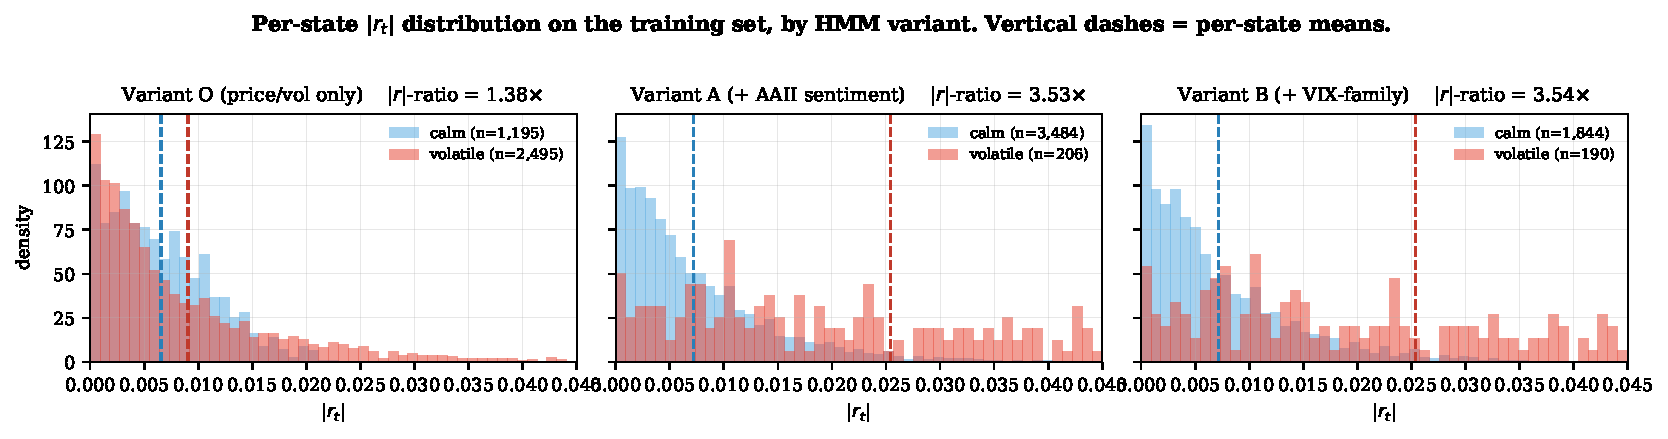
\includegraphics[width=\linewidth]{figures/F3_hmm_state_separation.pdf}
\caption{Per-state distribution of $|r_t|$ on the training set, by HMM variant. Variants A and B carve a tight ``crisis-spike detector'' partition; variant O's HMM, lacking sentiment, settles on a much milder ``activity-split'' that pools crises with normal high-activity trading. The same heavy concentration near $|r_t| = 0$ appears in every panel because absolute returns are non-negative and most days have small moves; this is a property of equity returns rather than of the HMMs.}
\label{fig:regime}
\end{figure}

\begin{figure}[H]
\centering
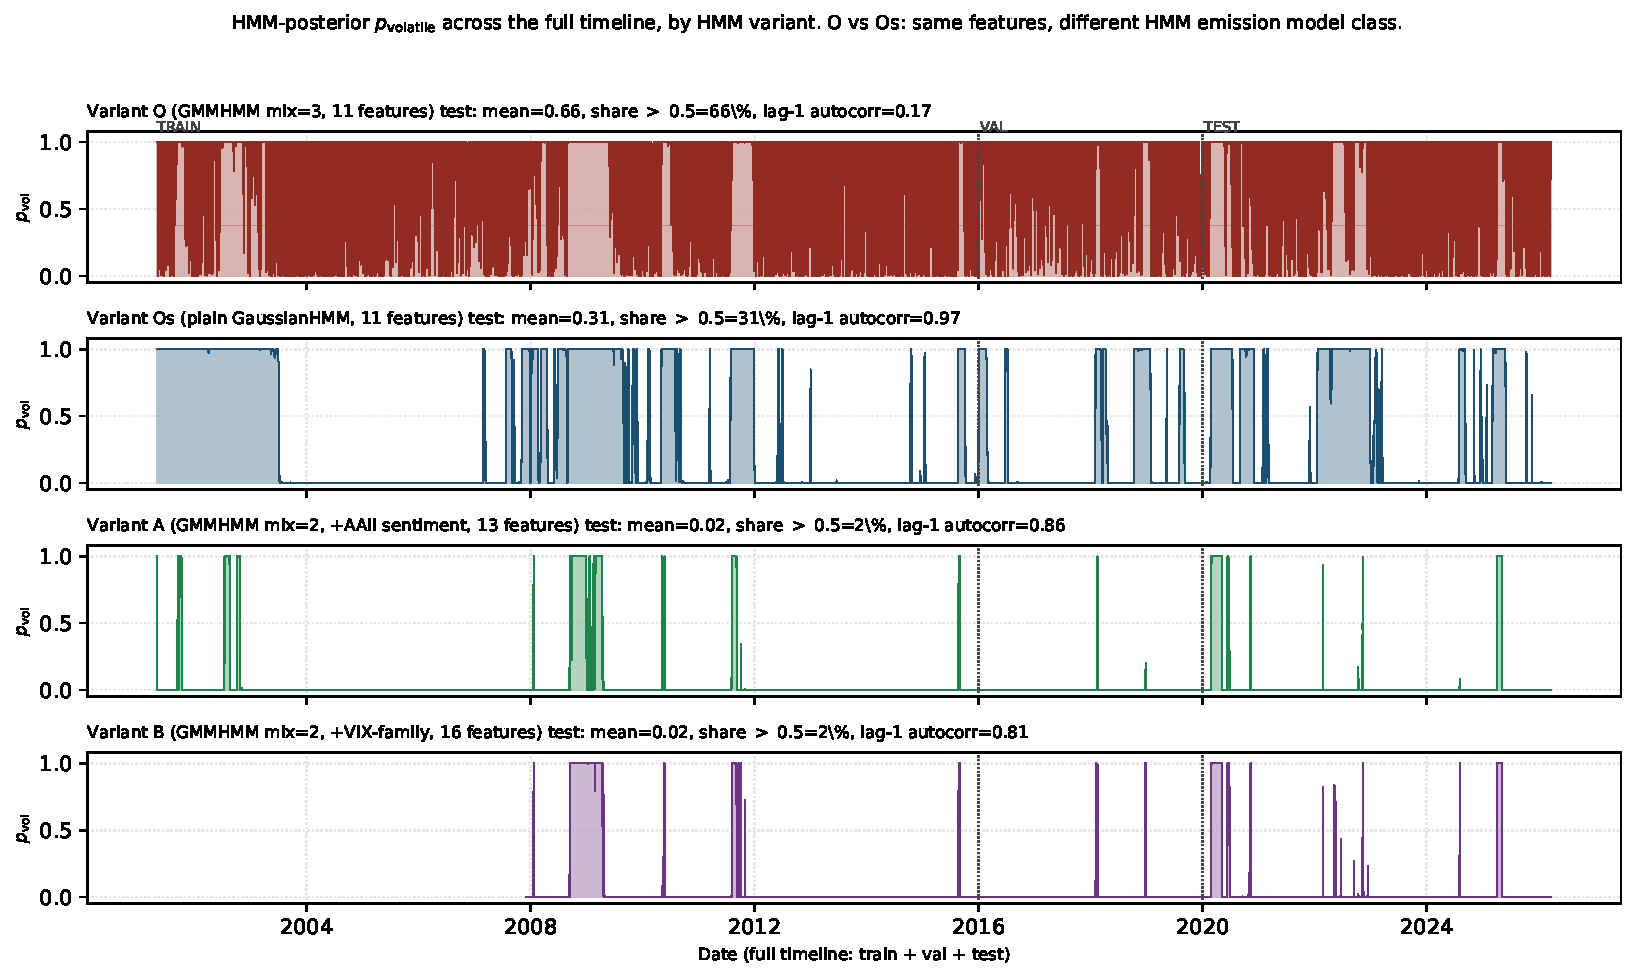
\includegraphics[width=\linewidth]{figures/F4_p_volatile_over_time.pdf}
\caption{HMM-posterior $p_{\mathrm{volatile}}$ across the full timeline (train + val + test, dotted lines mark split boundaries). Test-window summaries: variant O (top, GMMHMM) is persistently elevated and noisy (mean $0.66$, lag-1 autocorrelation $0.17$); variant Os (second, GaussianHMM on identical features, accessory probe) is clean and persistent (mean $0.31$, autocorrelation $0.97$); variants A and B sit near zero except during identifiable crisis intervals (means $0.02$ and $0.02$, autocorrelations $0.86$ and $0.81$). The O$\to$Os contrast on identical features is the methodological discovery of \cref{sec:os-discovery}.}
\label{fig:pvol}
\end{figure}

\subsection{Cross-seed variance disclosure}
\label{app:cv}

\begin{table}[H]
\centering
\caption{Cross-seed coefficient of variation (CV $=$ std~$/$~mean $\times 100\%$, $n=3$ seeds, sample std with $\mathrm{ddof}{=}1$) for each predictor.}
\label{tab:cv}
\small
\begin{tabular}{@{}lcccc@{}}
\toprule
Predictor & MSE CV \% & RMSE CV \% & MAE CV \% & MAPE CV \% \\
\midrule
variant O (ensemble) & $3.2$  & $1.6$  & $3.0$  & $3.8$  \\
variant A (ensemble) & $5.7$  & $2.8$  & $2.1$  & $5.8$  \\
variant H (baseline) & $6.7$  & $3.3$  & $1.9$  & $3.3$  \\
variant B (ensemble) & $\mathbf{13.5}$ & $\mathbf{6.7}$ & $\mathbf{6.3}$ & $6.4$ \\
\bottomrule
\end{tabular}
\end{table}

\subsection{Os/As/Bs accessory probe metrics}
\label{app:os-probe}

\begin{table}[H]
\centering
\caption{Three accessory pipelines (Os, As, Bs) vs their mixture-emission counterparts (O, A, B) on the common 1{,}440-row test index. Each pair shares features and LSTM hyperparameters; only the HMM emission differs (BIC-selected GMMHMM, with $n_{\mathrm{mix}}=3$ for O and $n_{\mathrm{mix}}=2$ for A and B, vs plain Gaussian). Lag-1 autocorrelation of $p_{\mathrm{volatile}}$ on test is shown as a regime-quality proxy.}
\label{tab:os-probe}
\small
\begin{tabular}{@{}lcccccc@{}}
\toprule
Predictor & RMSE & MAE & MAPE & MAPE $\Delta$ pair & autocorr & MAE CV \% \\
\midrule
variant O  (ens.) & $0.00378$ & $0.00264$ & $30.14\%$ & ---       & $0.17$ & $3.0$ \\
\textbf{variant Os (ens.)} & $0.00370$ & $0.00237$ & $\mathbf{23.48\%}$ & $\mathbf{-6.66}$ pp & $\mathbf{0.97}$ & $\mathbf{1.2}$ \\[2pt]
variant A  (ens.) & $0.00360$ & $0.00235$ & $24.23\%$ & ---       & $0.86$ & --- \\
variant As (ens.) & $0.00355$ & $0.00234$ & $24.01\%$ & $-0.22$ pp & $0.97$ & --- \\[2pt]
variant B  (ens.) & $0.00359$ & $0.00239$ & $25.51\%$ & ---       & $0.81$ & --- \\
variant Bs (ens.) & $0.00387$ & $0.00256$ & $25.71\%$ & $+0.20$ pp & $0.98$ & --- \\
\bottomrule
\end{tabular}
\end{table}

\subsection{GMMHMM vs GaussianHMM emission across O, A, B}
\label{app:emission-comp}

\begin{figure}[H]
\centering
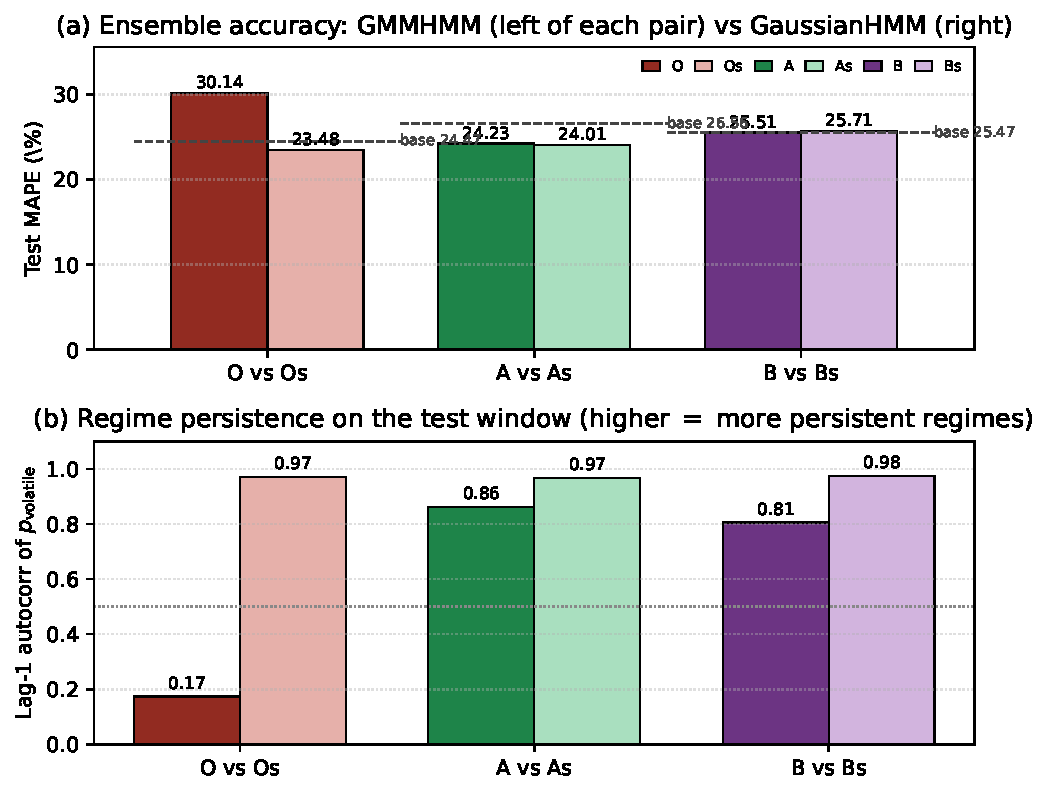
\includegraphics[width=\linewidth]{figures/F5_emission_comparison.pdf}
\caption{Three-way emission probe (variants O/A/B vs Os/As/Bs). \textbf{(a)} Test-set MAPE per pair; the dashed segments mark each pair's HMM-independent LSTM-only baseline. The O$\to$Os swap closes a $5.66$ pp gap to its baseline and overshoots it by $0.99$ pp; the A$\to$As and B$\to$Bs swaps are within $\pm 0.22$ pp. \textbf{(b)} Lag-1 autocorrelation of the test-window $p_{\mathrm{volatile}}$ posterior. Variant O's GMMHMM is the only degenerate fit (autocorr $0.17$); A and B are conservative-but-coherent (0.86, 0.81); all three GaussianHMM refits cluster near $0.97$. Together the panels show that the Os accuracy gain is a rescue of the broken O fit, not a generic GaussianHMM advantage.}
\label{fig:f5}
\end{figure}

\subsection{Variant Os HMM diagnostic: before/after comparison}
\label{app:os-diag}

\begin{figure}[H]
\centering
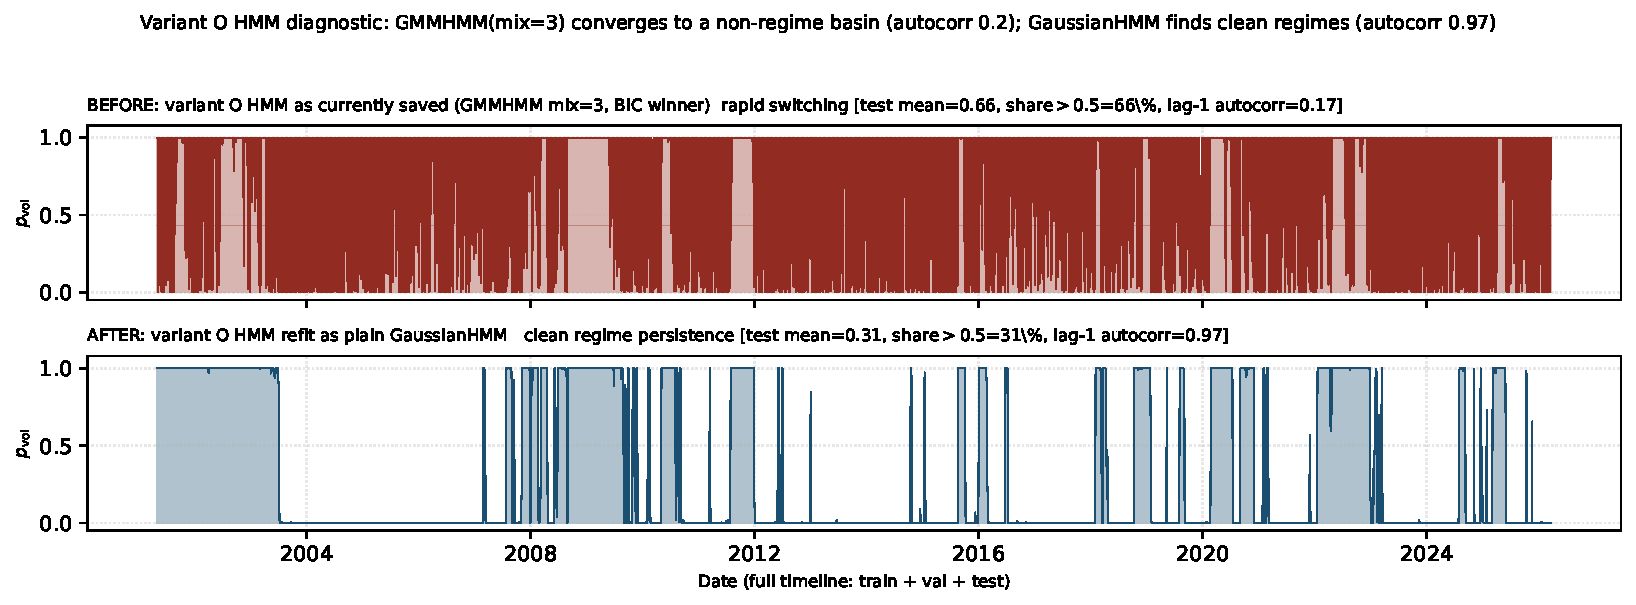
\includegraphics[width=\linewidth]{figures/F_variant_O_hmm_diagnostic.pdf}
\caption{Variant-O HMM diagnostic. \textbf{Top:} variant O as currently used (BIC-optimal $\mathrm{GMMHMM}(n_{\mathrm{mix}}=3)$); $p_{\mathrm{volatile}}$ flips between $0$ and $1$ on a near-daily basis, with lag-1 autocorrelation $\approx 0.17$ and $548$ flips above and below $0.5$ on the test window. \textbf{Bottom:} the same 11 features refit as a plain GaussianHMM (= variant Os), giving lag-1 autocorrelation $0.97$, $31$ flips, and persistent run-length structure consistent with volatility clustering. The duration-penalty sweep that motivated the refit is in \texttt{supplementary/diagnostics/variant\_O\_hmm\_sweep.csv}.}
\label{fig:variant-O-diag}
\end{figure}

\subsection{Reproducibility}

Code, executed notebooks (with output cells preserved), trained-model artefacts, prediction parquets, and per-seed predictions are at \url{https://github.com/maharajhaider/StockVolatilitySight}. The Colab bootstrap notebook \texttt{notebooks/colab\_bootstrap.ipynb} reproduces the full pipeline end-to-end on Colab free-tier CPU in approximately 95 minutes; the variant Os accessory pipeline is reproduced by \texttt{notebooks/colab\_variant\_Os\_refit.ipynb} and the variant As/Bs extension by \texttt{notebooks/colab\_variants\_AsBs\_refit.ipynb}.

\end{document}
